\documentclass{article}

\usepackage{graphicx}
\usepackage{tikz}
\usepackage{tikzsymbols}
\usetikzlibrary{calc,patterns,shapes.geometric}
\pagestyle{empty}
\usepackage[margin=0pt]{geometry}
\geometry{papersize={14in,12in}}

\def\centerarc[#1](#2)(#3:#4:#5){\draw[#1] ($(#2)+({#5*cos(#3)},{#5*sin(#3)})$) arc (#3:#4:#5);}

\begin{document}
	\begin{figure}
		\centering
		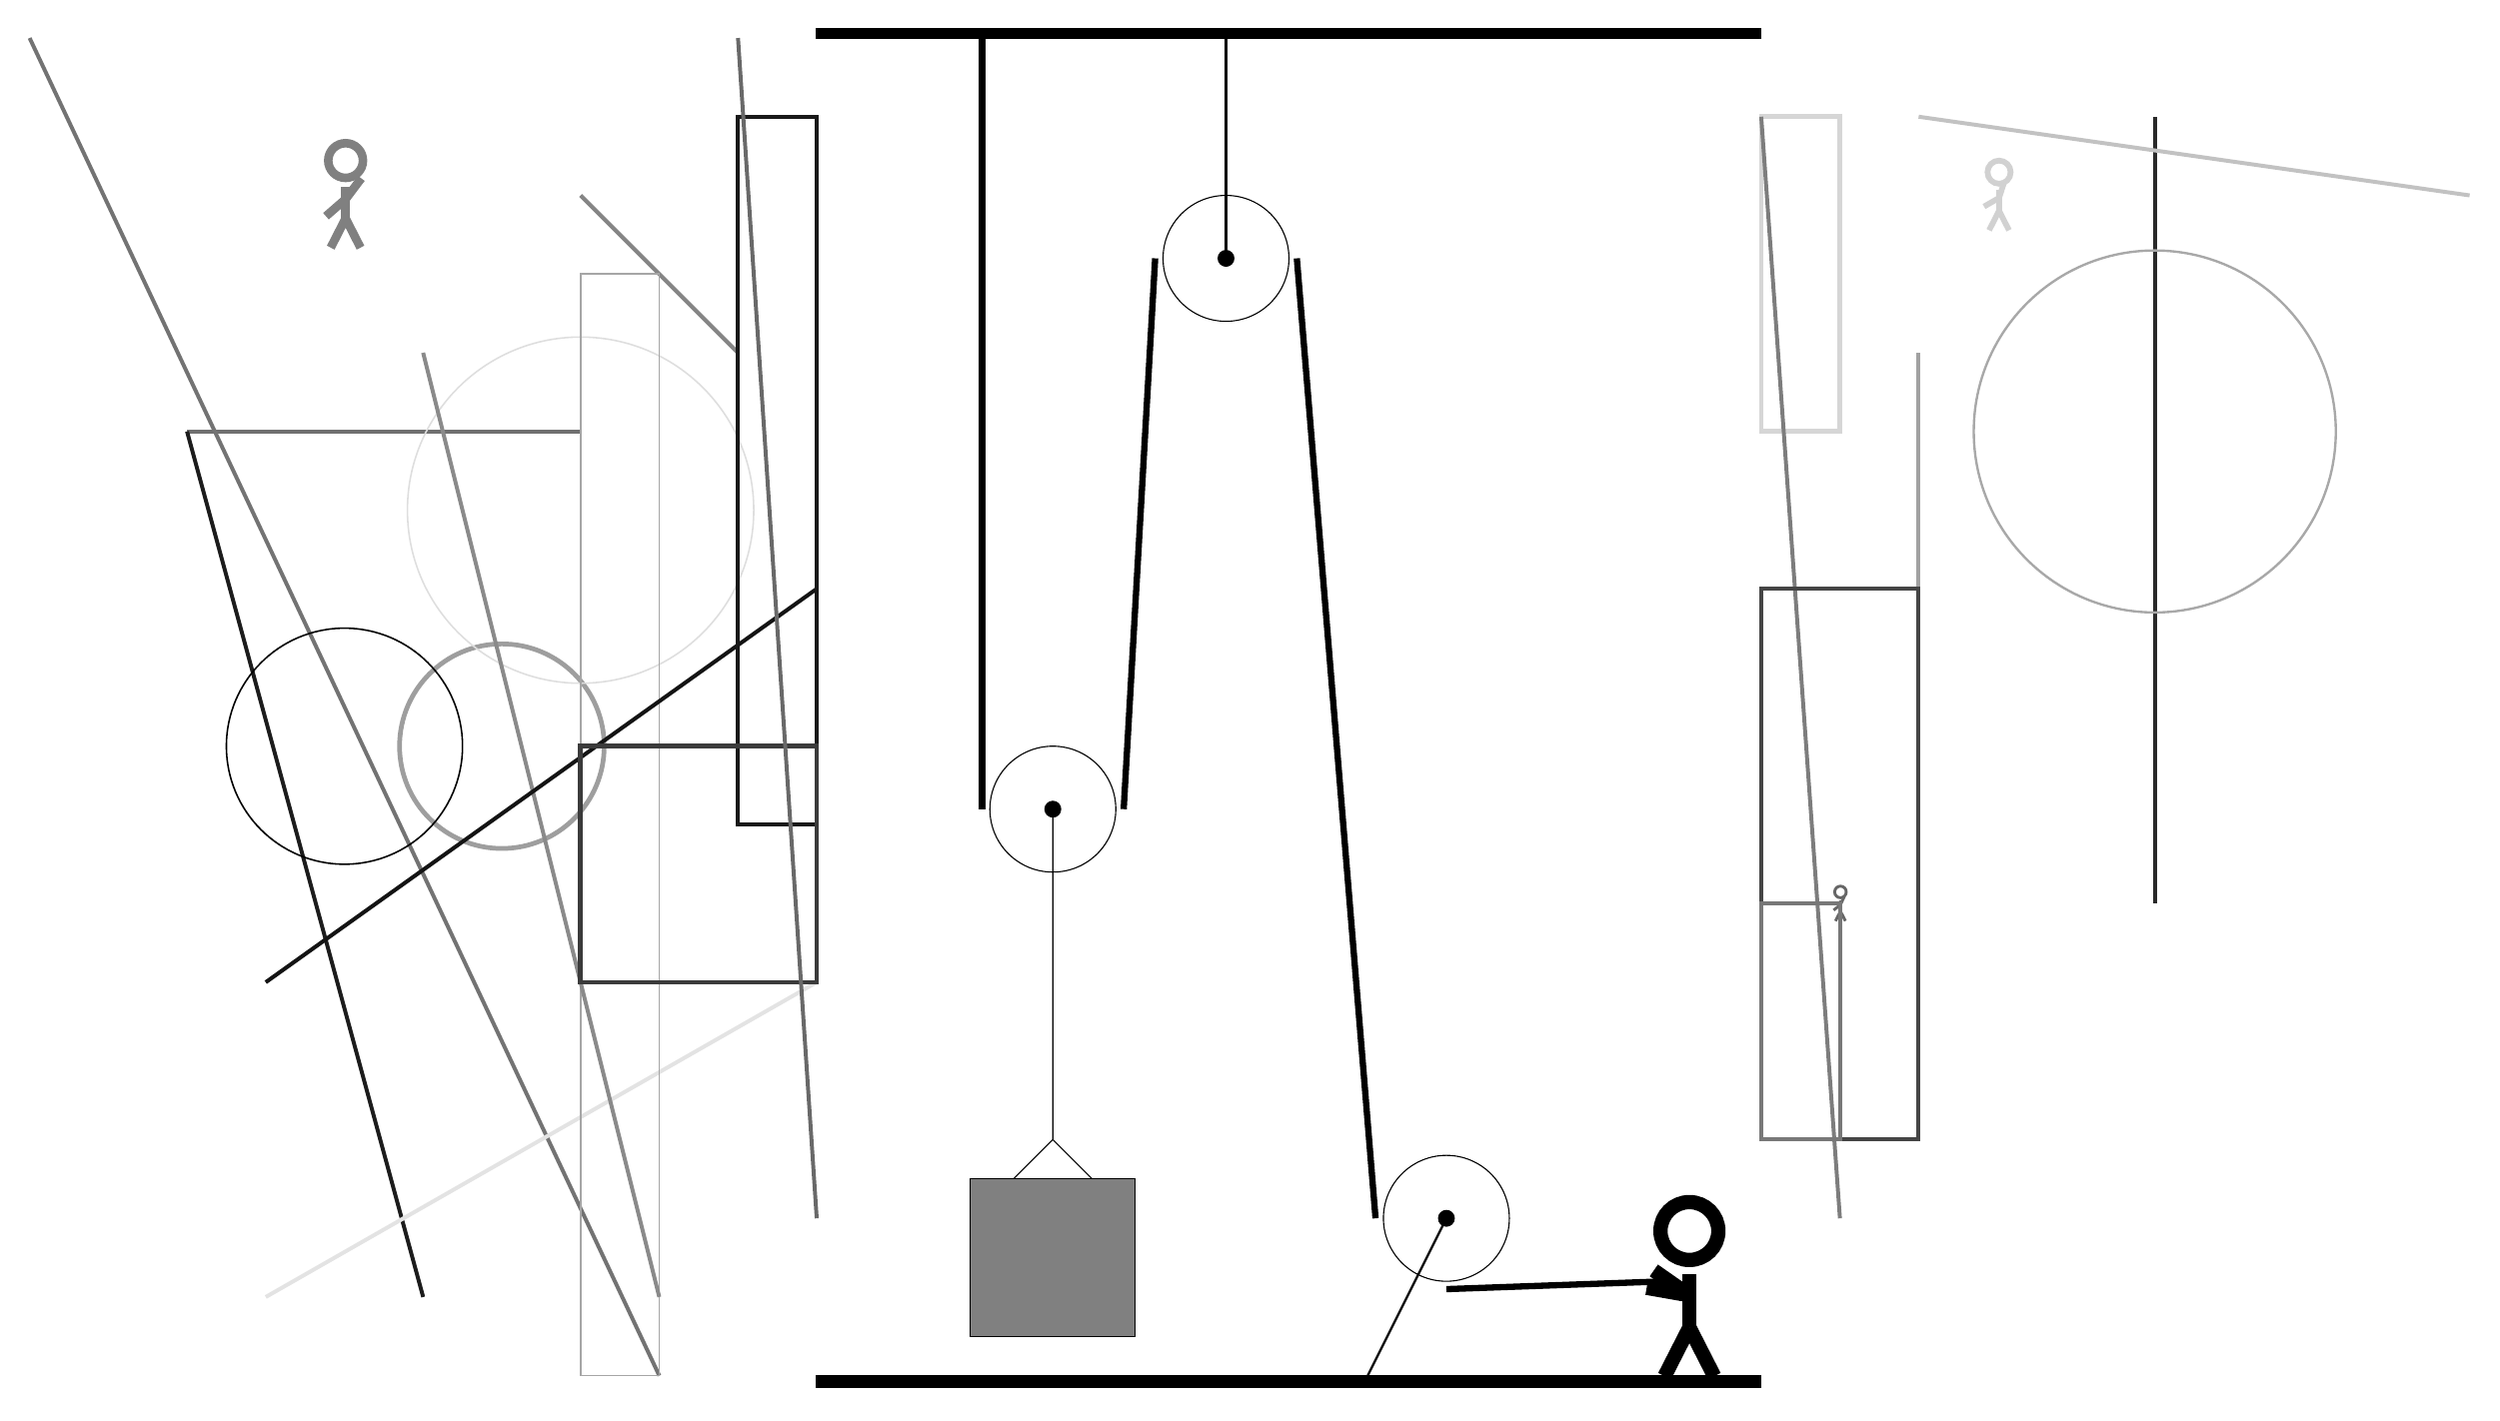
\begin{tikzpicture}
			%%%%% START %%%%%
			
			\draw[fill=black] (-2, 14) rectangle (10, 14.125);
			
			\draw (3.2, 11.2) circle (0.8);
			\draw[fill=black] (3.2, 11.2) circle (0.1);
			\draw[thick] (3.2, 11.2) -- (3.2, 14);
			
			\draw (6, -1) circle (0.8);
			\draw[fill=black] (6, -1) circle (0.1);
			\draw[thick] (6, -1) -- (5, -3);
			
			\draw (1, 4.2) circle (0.8);
			\draw[fill=black] (1, 4.2) circle (0.1);
			
			\draw (1, 4.2) -- (1, 0) -- (0.5, -0.5);
			\draw (1, 0) -- (1.5, -0.5);
			\draw[fill=black!50] (-0.05, -0.5) rectangle (2.05, -2.5);
			
			\draw[line width=0.8mm] (0.1, 14) -- (0.1, 4.2);
			\centerarc[line width=0.8mm](1, 4.2)(180:360:0.9);
			\draw[line width=0.8mm](1.9, 4.2) -- (2.3, 11.2);
			\centerarc[line width=0.8mm](3.2, 11.2)(0:180:0.9);
			\draw[line width=0.8mm](4.1, 11.2) -- (5.1, -1);
			\centerarc[line width=0.8mm](6, -1)(180:270:0.9);
			\draw[line width=0.8mm](6, -1.9) -- (8.8, -1.8);
			
			\draw[line width=0.6mm, color=black!16] (11, 9) rectangle (10, 13);
			
			\draw[line width=0.5mm, color=black!56](-5, 9) -- (-10, 9);
			\draw[line width=0.5mm, color=black!84](15, 13) -- (15, 3);
			\draw[line width=0.5mm, color=black!89](-7, -2) -- (-10, 9);
			
			\node[line width=0.6mm, color=black!50] at (-8, 12) {\Strichmaxerl[6][41][53]};
			
			\draw[line width=0.5mm, color=black!51](11, -1) -- (10, 13);
			
			\draw[line width=0.5mm, color=black!55](-4, -3) -- (-12, 14);
			
			\draw [line width=0.6mm, color=black!38](-6, 5) circle (1.3);
			\draw [line width=0.3mm, color=black!34](15, 9) circle (2.3);
			\node[line width=0.4mm, color=black!60] at (11, 3) {\Strichmaxerl[2][38][65]};
			\draw[line width=0.5mm, color=black!24](12, 13) -- (19, 12);
			
			\draw [line width=0.2mm, color=black!13](-5, 8) circle (2.2);
			\draw[line width=0.5mm, color=black!48](-5, 12) -- (-3, 10);
			\draw[line width=0.5mm, color=black!11](-2, 2) -- (-9, -2);
			\draw[line width=0.5mm, color=black!37] (12, 6) rectangle (12, 10);
			\draw[line width=0.2mm, color=black!35] (-4, -3) rectangle (-5, 11);
			\draw[line width=0.5mm, color=black!73] (12, 0) rectangle (10, 7);
			
			\node[line width=0.6mm, color=black!18] at (13, 12) {\Strichmaxerl[4][30][72]};
			\draw[line width=0.5mm, color=black!53] (10, 0) rectangle (11, 3);
			\draw[line width=0.5mm, color=black!46](-7, 10) -- (-4, -2);
			\draw [line width=0.2mm, color=black!100](-8, 5) circle (1.5);
			
			\draw[line width=0.5mm, color=black!92](-2, 7) -- (-9, 2);
			
			\draw[line width=0.5mm, color=black!90] (-2, 4) rectangle (-3, 13);
			\draw[line width=0.6mm, color=black!77] (-2, 2) rectangle (-5, 5);
			\draw[line width=0.5mm, color=black!59](-3, 14) -- (-2, -1);
			
			
			\node at (9, -1.9) {\Strichmaxerl[10][-35][170]};
			
			\draw[fill=black] (-2, -3) rectangle (10, -3.15);
			
			%%%%% END %%%%%
		\end{tikzpicture}
	\end{figure}	
\end{document}